fAprès avoir identifié les \textit{exempla} dans SourcEncyMe et les encyclopédies dans ThEMA, il a été nécessaire de créer des connexions entre les deux bases de données. Pour ce faire, j’ai d'abord indexé les \textit{exempla} identifiés dans SourcEncyMe en les regroupant dans un recueil factice où les liens pouvaient être ajoutés. Ensuite, j'ai développé un code permettant d'ajouter des liens vers les \textit{exempla} qui contiennent des références à des \index{Encyclopédies}encyclopédies.


\section{Indexation des \textit{exempla} de SourcEncyMe dans ThEMA}
Une fois les \index{Récits exemplaires}récits exemplaires repérés dans SourcEncyMe, il était essentiel de les connecter à ThEMA. La question s’est posée de savoir où et comment les placer dans la base de données. L'équipe de SourcEncyMe envisageait de créer des entrées d’\textit{exempla} directement dans ThEMA en y ajoutant les informations pertinentes. Cependant, cette approche ne correspondait pas au fonctionnement de ThEMA, où les \textit{exempla} sont toujours intégrés dans un recueil spécifique, respectant ainsi le contexte et l’auteur d'origine.

Avec l'accord d'\index{Isabelle Draelants}Isabelle Draelants et de \index{Marie-Anne Polo de Beaulieu}Marie-Anne Polo de Beaulieu, nous avons décidé de créer un recueil intitulé « \textit{Exempla} de [Nom de l'encyclopédie] ». Cette solution s'inscrivait dans la vision de ThEMA, qui se veut une base de données d’œuvres contenant des \textit{exempla}, sans se limiter aux seuls recueils d'\textit{exempla}. De plus, lors de l'indexation, nous avons choisi d’inclure un extrait du texte en latin de l'\textit{exemplum} trouvé dans l'encyclopédie dans le champ : « texte original ». Cependant, étant donné que le texte des \index{Encyclopédies}encyclopédies est encore en cours de révision, il a été convenu que ces extraits seraient éventuellement supprimés pour éviter la diffusion de versions incorrectes. À l'avenir, des chercheurs ou des étudiants seront chargés de finaliser l'indexation en créant des résumés et en ajoutant des mots-clés, après quoi les extraits en latin seront retirés. L'indexateur pourra également supprimer un \textit{exemplum} s'il estime qu'il n'en est pas véritablement un, car il ne faut pas oublier qu'une partie des \textit{exempla} a été identifiée automatiquement par un algorithme. Dans ce cas, il devra simplement contacter l'équipe de SourcEncyMe pour qu'ils mettent à jour le lien de leur côté.

Pour intégrer les \textit{exempla} dans ThEMA, j'avais initialement envisagé d’utiliser un code \index{Python}Python ou \index{XQuery}XQuery pour générer les fichiers \index{XML}XML des \textit{exempla}. Ils auraient recréé le schéma \index{XML}XML des \textit{exempla} de ThEMA et il aurait juste fallu réintégrer les XML des \index{Récits exemplaires}récits exemplaires dans la base pour qu'ils apparaissent. Mais j’ai finalement opté pour une solution différente. J’ai développé un script \index{Python}Python de web scraping (annexe I) qui tire parti de l'interface de création d'\textit{exempla} déjà existante dans la base de données. Ce script se connecte à la base de données locale, navigue dans le recueil créé, crée chaque \textit{exemplum}, y insère le texte source, et répète l’opération pour chaque \textit{exemplum} repéré.  Le code cible plus spécifiquement toute les <ref', target="\#exemplum"> et récupère le texte dans la balise <quote> en dessous. Le code ne cible par le marqueur \textit{exemplum} car il n'est pas toujours présent même si un \textit{exemplum} est dans le texte. Cette méthode a l’avantage de créer directement les \textit{exempla} dans la base, sans avoir à charger manuellement les fichiers XML, réduisant ainsi les risques d'erreurs.

Ce code pourra être réutilisé à l'avenir pour accélérer l'indexation des textes dans ThEMA, à condition que les \textit{exempla} soient préalablement balisés. Il pourrait également être amélioré en intégrant un module capable de générer automatiquement des mots-clés pour les résumés, ce qui rendrait le processus d'indexation encore plus rapide.


\section{Gestion des liens vers SourcEncyMe dans ThEMA}
\subsection{Création des liens}
Lors de l'intégration des liens dans mon code, j'ai rencontré un problème. Le créateur d'\textit{exempla} de la base ThEMA possède un champ spécifique pour ajouter ces liens, mais ce champ est « dynamique ». Cela signifie que la page peut se modifier ou réagir aux actions de l'utilisateur sans nécessiter un rechargement complet. Cependant, mon code ne parvenait pas à interagir correctement avec cette partie dynamique, qui permet d'ajouter ou de supprimer des liens. \\
 
 \begin{figure}[H]
 	\centering
 	\fbox{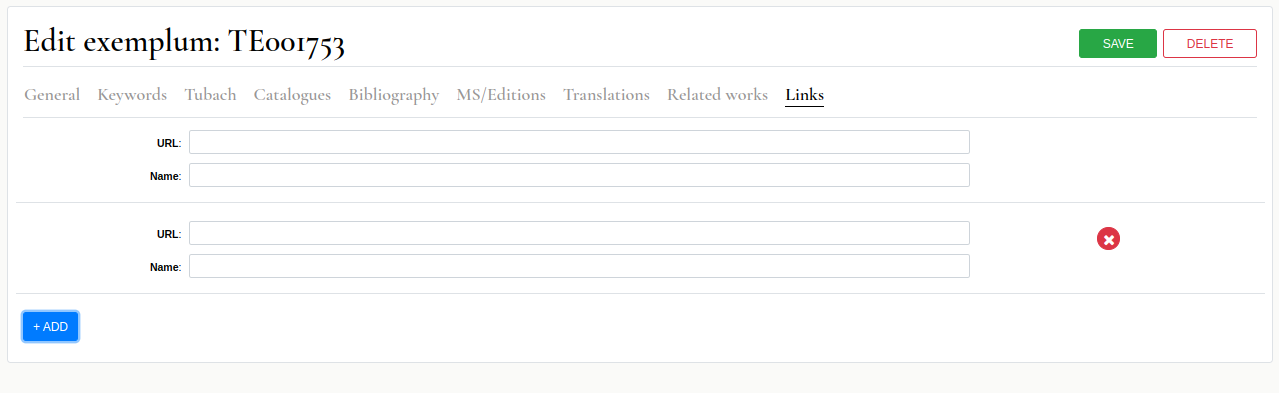
\includegraphics[width=0.5\linewidth]{images/champlienthema.png}}
 	\caption{Page dynamique pour ajouter des liens dans ThEMA}
 \end{figure}

Finalement, il a été nécessaire de développer un script \index{Python}Python pour modifier les fichiers XML et y ajouter les liens (annexe J). Pour cela, j'ai dû télécharger le dossier contenant les \textit{exempla} de Giovanni da San Gimignano. Le script vérifie d'abord que le texte dans les \index{XML}XML de ThEMA correspond bien à celui dans SourcEncyMe. Une fois cette vérification effectuée, le lien vers SourcEncyMe est ajouté dans les \index{XML}XML de ThEMA, et dans les \index{XML}XML de SourcEncyMe. Les liens sont construits comme suit : \\

 \begin{figure}[H]
	\centering
	\fbox{
\includegraphics[width=0.8\linewidth]{images/lienthemaexemple.png}}
	\caption{Exemple de lien vers ThEMA}
\end{figure}

Pour accéder aux exempla, la base ThEMA passe d'abord par Huma-Num qui héberge la base. Ensuite, elle interroge le fichier « exempla.xql » pour afficher les \textit{exempla} sous forme de contenu web. Enfin, elle appelle le fichier \index{XML}XML correspondant à l'\textit{exemplum} créé dans ThEMA. \\

\begin{figure}[H]
	\centering
	\fbox{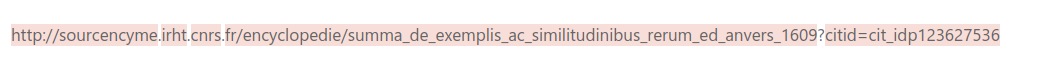
\includegraphics[width=0.8\linewidth]{images/linksourcencymeexemple.png}}
	\caption{Exemple de lien vers SourcEncyMe}
\end{figure}

Pour accéder aux citations d'\index{Encyclopédies}encyclopédies, la base SourcEncyMe passe par l'IRHT et le CNRS, qui hébergent la base de données. Ensuite, elle interroge le fichier gérant les encyclopédies et leur affichage web. Enfin, elle appelle une encyclopédie spécifique et une citation précise identifiée par un code cit\_id, unique pour chaque citation, trouvé dans la balise <cit> : \\

 \begin{figure}[H]
	\centering
	\fbox{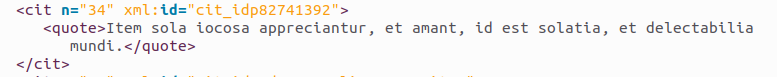
\includegraphics[width=0.8\linewidth]{images/citidsourcenycme.png}}
	\caption{Localisation du cit\_id dans SourcEncyMe}
\end{figure}

Avant de créer les liens, j'ai vérifié auprès des deux équipes si les identifiants resteraient constants dans le temps pour garantir la pérennité des liens.


\subsection{Perspectives pour la création du lien}
Dans une perspective d'amélioration future, j'ai envisagé de modifier le champ d'ajout de liens pour qu'il fonctionne de manière similaire aux autres champs contenant des données préenregistrées. L'objectif serait de préenregistrer tous les liens vers SourcEncyMe, afin d'éviter aux chercheurs de les copier manuellement et de supprimer la nécessité de modifier directement les fichiers \index{XML}XML à l'aide d'un script \index{Python}Python.

J'avais envisagé d'apporter des modifications à l'interface de balisage XMLmind, utilisée pour baliser les \index{Encyclopédies}encyclopédies de SourcEncyMe. Cependant, je n'ai pas eu le temps de m'en occuper, et c'est finalement \index{Emmanuelle Kuhry}Emmanuelle Kuhry qui s'est proposée de s'en charger. Il sera nécessaire d'adapter la fenêtre pop-up permettant de sélectionner une œuvre pour une citation dans XMLmind, en y ajoutant des liens vers les \textit{exempla} de la base et la classification de Tubach.


\section{Création de liens vers SourcEncyMe depuis les mentions d'encyclopédies dans ThEMA}
Pour ajouter des liens entre les \textit{exempla} et les références à des \index{Encyclopédies}encyclopédies, j'ai utilisé un script \index{Python}Python (annexe K) qui explore les fichiers \index{XML}XML de la base téléchargée sur mon ordinateur. Le script recherche des mentions d'encyclopédies en utilisant une expression régulière spécifiée pour chaque encyclopédie. Par exemple, pour le \index{Speculum historiale}\textit{Speculum historiale}, l'expression régulière utilisée est : \\

\begin{verbatim} r'S?s?peculum historiale,? ([IVXLCDM]+|\d+)[.,]?\s*([0-9]+)?' \end{verbatim}

\

Cette expression régulière est conçue pour détecter les références au texte \index{Speculum historiale}\textit{Speculum historiale}, en tenant compte des variations possibles dans l'usage des majuscules, ainsi que des numéros de volume en chiffres romains ou arabes. Le script continue en récupérant les numéros de chapitre mentionnés et en cherchant ces numéros dans le fichier \index{XML}XML de l'\index{Encyclopédies}encyclopédie. Une fois le numéro de chapitre trouvé, il est converti en chiffre arabe si nécessaire. Le script récupère ensuite le cit\_id correspondant et l'insère dans un lien préétabli au nom de l'encyclopédie (à ajuster par l'utilisateur), puis intègre ce lien dans le \index{XML}XML de ThEMA. Finalement, le script place l'identifiant TE... dans le champ cit du \index{XML}XML, car il s'agit d'un élément repris et non d'un \textit{exemplum}, ce qui évite l'identification d'une œuvre.

Cependant, plusieurs problèmes ont été rencontrés lors de l'exécution de ce code. Premièrement, l'extraction des mentions d'\index{Encyclopédies}encyclopédies s'est révélée compliquée en raison de l'utilisation mixte d'indexations en texte intégral et d'attributs récupérés lors du chargement de la page web de la base de données. Les attributs spécifiques associés aux encyclopédies, stockés dans le fichier list\_bibliography.xml, sont : \\

\begin{center}
\begin{tabular}{|c|c|}
	\hline
	Z-S7UCXT48 & \index{Speculum naturale}\textit{Speculum naturale} \\
	\hline
	Z-38N6WX3E & \index{Speculum historiale}\textit{Speculum historiale}  \\
	\hline
	Z-D6KRQBMP & \textit{Liber de natura rerum} \\
	\hline
\end{tabular}
\end{center}

\

Le script devait donc non seulement effectuer des recherches en texte intégral mais aussi intégrer et traduire ces codes avant de réaliser les recherches en texte intégral. Voilà à quoi ressemble un cas de mention plein texte d'encyclopédie dans un XML de ThEMA et une mention d'encyclopédie liée à un attribut : \\

\begin{lstlisting}[breaklines=true]
<sourceDesc>
	<list type="source_details">
		<item type="source_text"><p/></item>
		<item type="sources"><p>Vincent de Beauvais, Speculum naturale, 16, 97 (Douai, 1624, col. 1213).</p></item>
		<item type="exemplum_context"><p>III, tit. VI, De peregrinatione</p></item>
		<item type="commentary"><p/></item>
		<item type="allegory">n</item>
	</list>
\end{lstlisting}

\begin{lstlisting}[breaklines=true]
<listBibl>
	<bibl type="tubach" corresp="Z-WLZ7CBVC" n="TUB3969"/>
	<bibl type="related_texts" corresp="" n="">Valerius Maximus, Dictorum factorumque memorabilium libri novem..., V, c.4.7.ext.</bibl>
	<bibl type="related_texts" corresp="Z-38N6WX3E" n="6, 125"/>
	<bibl type="related_texts" corresp="" n="">British Library, Add. 33956 [transcr. Welter], 427</bibl>
	<bibl type="related_texts" corresp="" n="">Liber ad status [Paris, BnF, ms. lat. 6368], 4,21</bibl>
\end{lstlisting}

\begin{lstlisting}[breaklines=true]
<biblStruct xml:id="Z-38N6WX3E" type="book" corresp="#http://zotero.org/groups/2304628/items/38N6WX3E">
	<monogr>
		<title level="monograph">Speculum historiale</title>
		<title level="short"/>
		<author>
			<name>Vincentius Belvacensis</name>
		</author>
		<imprint>
			<pubPlace>Douai</pubPlace>
			<date type="pub_date">1624</date>
		</imprint>
	</monogr>
</biblStruct>
\end{lstlisting}

\

Un autre problème rencontré concernait la différence entre les numéros de chapitres indexés dans ThEMA et ceux présents dans SourcEncyMe. Les numéros de chapitres utilisés par les indexateurs pour le \textit{Speculum historiale} sont basés sur l'édition de 1624, tandis que le classement de SourcEncyMe est décalé d'un numéro\footnote{Vincent de Beauvais, \textit{Speculum historiale}. \textit{Bibliotheca mundi Vincentii Burgundi, ex ordine Praedicatorum venerabilis episcopi Bellovacensis, Speculum quadruplex, naturale, doctrinale, morale, historiale}, Douai, ex officina typographica Baltazaris Belleri, 1624.}. Ainsi, chaque fois que le code récupère un numéro de chapitre de ThEMA, il doit ajouter un à ce numéro pour correspondre à SourcEncyMe. Par exemple, pour l'\textit{exemplum} 844 de la \textit{Scala Coeli}, les indexateurs ont mentionné le chapitre 26, 32, alors que dans SourcEncyMe, ce textes se trouve au chapitre 27, 33. \\

 \begin{figure}[H]
	\centering
	\fbox{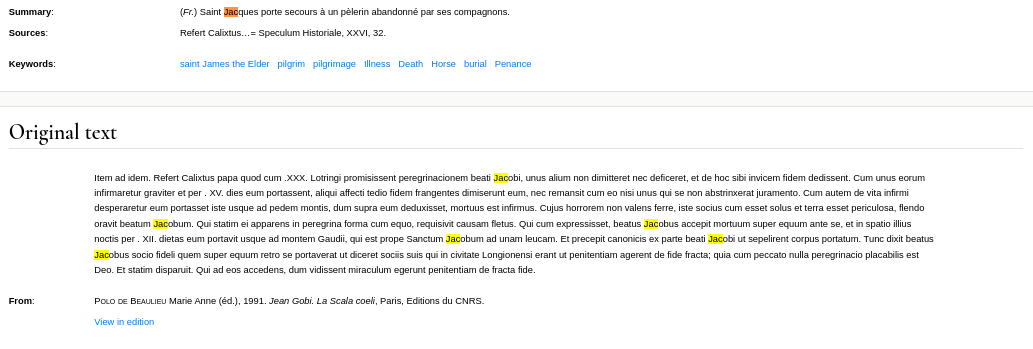
\includegraphics[width=0.8\linewidth]{images/problemnumero1.png}}
	\caption{Récit exemplaire reprenant un texte encyclopédique}
\end{figure}

 \begin{figure}[H]
	\centering
	\fbox{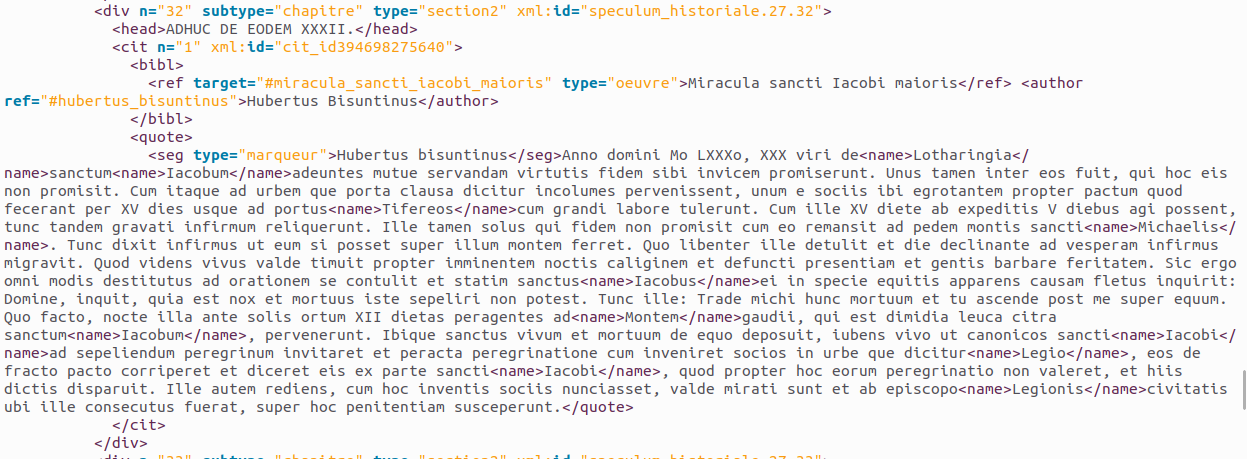
\includegraphics[width=0.8\linewidth]{images/problemnumero2.png}}
	\caption{Texte de l'encyclopédie qui est repris}
\end{figure}

Le dernier problème a résidé dans la division des \index{Encyclopédies}encyclopédies en citations. Les liens peuvent uniquement être créés pour des citations spécifiques, alors que les numéros de chapitres indexés dans ThEMA ne fournissent que le numéro de chapitre, tandis qu'il peut y avoir plusieurs citations pour un même chapitre. Après discussion avec \index{Emmanuelle Kuhry}Emmanuelle Kuhry et \index{Isabelle Draelants}Emmanuelle Kuhry, il a été décidé de placer les liens dans la première citation de chaque chapitre. Cette approche laisse à l'utilisateur le soin de trouver le passage exact. Cette solution a été retenue en raison de la complexité et du volume de vérifications manuelles nécessaires, étant donné que parfois un passage peut être mentionné dans toutes les citations d'un chapitre ou seulement dans une seule.